\newlength{\taskspace}
\setlength{\taskspace}{-.2in}

%TODO for colorblind access, label green and red filters as such

\chapter{Spectrum of black body radiation}

\section{Introduction}

In this lab you will study the continuous emission of bodies heated to a particular temperature. Such emission can be compared to that of an idealized ``blackbody,'' a term introduced by physicist Gustav Kirchhoff in 1860. A blackbody perfectly absorbs all incident radiation, and thus would appear perfectly black. At the same time, it emits continuous radiation with a spectrum that peaks at a wavelength inversely proportional to the body's temperature.

Although the term may sound mysterious, you see sources of such radiation every day all around you. Incandescent light bulbs that are still commonly used for lighting emit a spectrum very close to that of an ideal blackbody, as you will see in this lab. The Sun light that we enjoy every day also has a spectrum that can be approximated by the blackbody spectrum. Likewise, stars that you see in the night sky emit light with spectra that can be approximated by blackbody spectra. You will check this in this lab for spectra of a few representative stars. This lab also illustrates a very important concept. Physical sciences in general, and astronomy in particular, achieved significant progress because physical laws discovered here and now in the lab turn out to be universally applicable. Thus, for example, you can study Balmer lines of hydrogen from a discharge tube in the lab and then find similar lines in spectra of stars or galaxies. It is this universality that makes science tick. It would be very difficult for us to make sense of astronomical objects, if they worked according to their own
celestial laws, not accessible to study in our terrestrial labs. (Yet, this was the accepted view until the scientific revolution of 16th--17th centuries).

In this lab you will employ this powerful concept by first learning how to measure the temperature of a tungsten filament in an incandescent bulb: you will measure the bulb blackbody-like light spectrum with the Red Tide spectrometer, and then apply the same technique to calculate the surface temperature of stars from their spectra.

\section{Black body spectrum and the Planck formula}

The blackbody spectrum has a shape characterized by a broad peak. The peak wavelength position is inversely proportional to the temperature of a blackbody emitting the radiation.  This is known as Wein's Law:

\begin{equation}\label{bb:eq:lmax}
\lambda_\textrm{max} = 2.9\times 10^6\,\textrm{nm/T}
\end{equation}

\renewcommand{\theenumi}{\thesection.\arabic{enumi}}
%\renewcommand{\theenumi}{\thesubsection.\arabic{enumi}}


\textbf{Lab tasks.}
%\vspace{\taskspace}
 
	\begin{enumerate}
		\item \textbf{We are all blackbody emitters!  Estimate the peak emission wavelength for a normal body temperature of 310 K.  Which part of the electromagnetic spectrum does this correspond to?}
	\end{enumerate}


\begin{figure}[htb]
	\begin{center}
		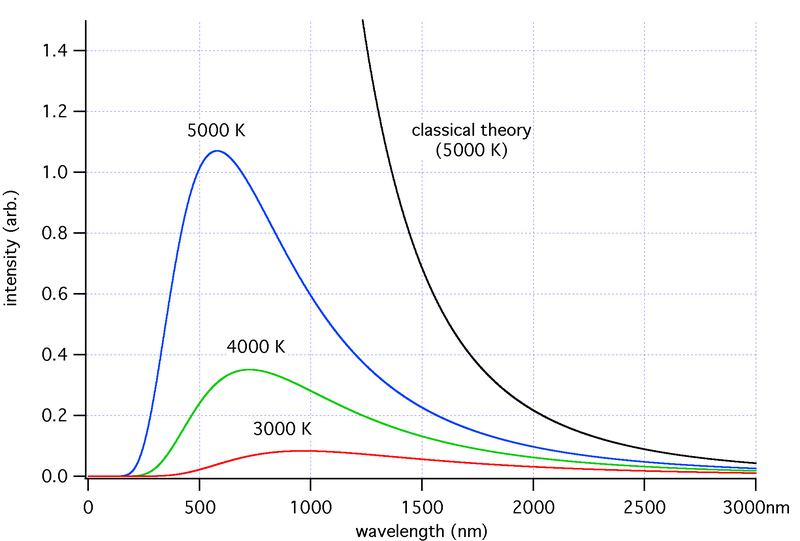
\includegraphics[angle=0,width=0.6\textwidth]{blackbody/planck01.jpg}
		\caption{\label{bb:fig:planck}
			The spectrum of radiation emitted by a perfect blackbody at temperatures of 3000K, 4000K, and 5000K according to the Planck formula is shown by red, green, and blue lines, respectively. The solid black line shows prediction of classical (non-quantum) thermodynamics for emission at 5000K
			%, which is quite different from the Planck formula. It is the Planck formula that describes experimental results and not the classical formula. This discrepancy was one of the
			%main factors that led to development of quantum mechanics that superseded classical theory. 
			(Figure source: Wikipedia.org).}
	\end{center}
\end{figure}

The shape of the blackbody spectrum was measured in laboratory at the end of 19th century and was a source of much puzzlement to the physicists of that time because it contradicted the expectations of classical thermodynamics (the branch of physics studying heat and radiation). Attempts to understand the shape of the blackbody spectrum led to development of quantum mechanics. The formula accurately describing the shape of the measured spectrum was proposed by the German physicist Max Planck in 1900. Planck also showed how this shape can be understood using theoretical calculations based on concepts of quanta of energy and thermodynamic equilibrium. The Planck formula describing the shape of the blackbody spectrum as a function of wavelength $\lambda$ is given by the following formula:

\begin{equation}\label{bb:eq:planck}
B_\lambda (T) = \frac{2 h c^2}{\lambda^5} \frac{1}{\exp(\frac{h c}{\lambda k T}) - 1}
\end{equation}
where $h=6.63\times10^{-34}\,$J/s is the Planck constant, $c=2.99\times 10^8\,$m/s is the speed of light in vacuum, and $k=1.38\times 10^{-23}\,$J/K is the Boltzmann constant.  The Planck spectrum shape for different temperatures along with predictions of the classical theory is shown in Fig.~\ref{bb:fig:planck}.% Note that often the entire spectrum cannot be measured due to limited spectral coverage of equipment. In this case one can measure a portion of the spectrum and still compare it to the blackbody spectrum, as you will see in this lab.

\begin{figure}[htb]
	\begin{center}
		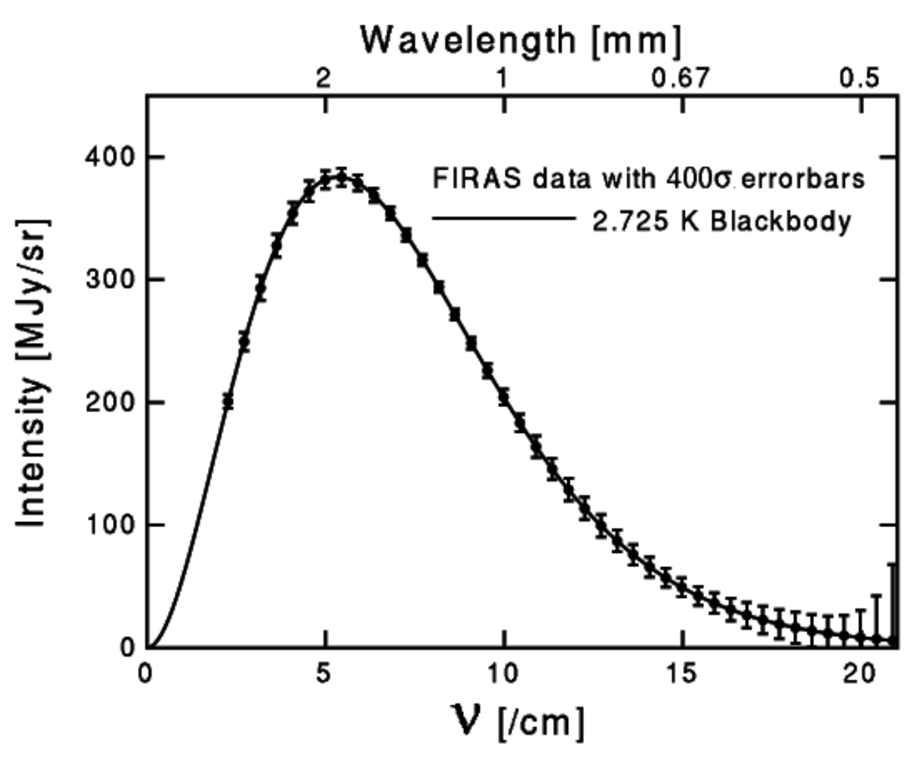
\includegraphics[angle=0,width=0.6\textwidth]{blackbody/firas_spectrum.pdf}
		\caption{Spectrum of CMB as measured by the FIRAS instrument on COBE satellite in the 1990s. Note that the measured spectrum is described almost perfectly by the Planck formula with an effective temperature of 2.7K; the error bars shown are $400 \sigma$!}\label{bb:fig:cobe}
	\end{center}
\end{figure}

Fig.~\ref{bb:fig:cobe} shows the spectrum of the CMB radiation -- a ubiquitous relic radiation from the first few thousand years in the existence of our universe. This radiation was emitted when the universe was very hot and dense and almost in thermodynamic equilibrium. The spectrum is thus very accurately approximated by the Planck formula. %You will measure the CMB radiation and its temperature in one of the labs in PhySci 120 course next quarter. 
Note that this is yet another example of the amazing universality of physical laws in nature. You can use the same formula to describe the spectrum of a regular incandescent bulb and spectrum of relic radiation from the early era of evolution of our universe!

\section{Experimental setup}
\subsection{Spectrometer hardware}

In this lab we will use the the Ocean Optics digital spectrometer, which measures light in the range 350 to 1000 nm with a resolution of about $1\,$nm  ($1\,\textrm{nm} = 10^{-9}\,\textrm{m}$.) Light from the source under study is collected by an optical fiber. \textbf{IMPORTANT: the fiber is fragile, handle with care.} The fiber will be fixed in a holder, which can be adjusted to point to the light bulb. The spectrometer is connected to the computer through USB, and dedicated software (Spectra Suite) is used to operate the spectrometer and save the data. For reference, Fig.~\ref{bb:fig:software1} shows the main controls of the SpectraSuite software.

You will use a regular 25W incandescent light bulb setup in a holder, with a voltage regulator to change the light intensity.

\begin{figure}
	\begin{center}
		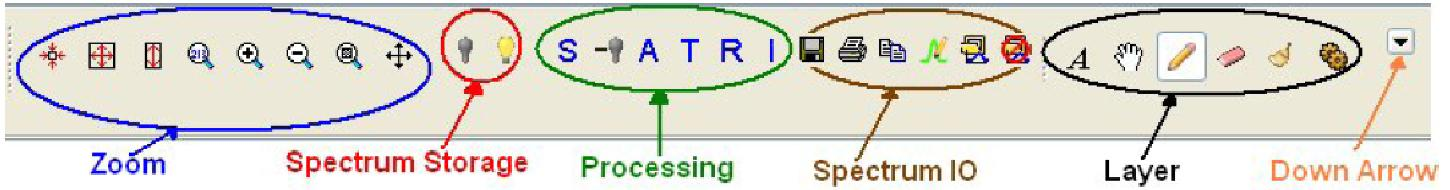
\includegraphics[angle=0,width=1.0\textwidth]{blackbody/software1.jpg}
		\caption{The Spectra Suite software controls: zoom controls can be used to zoom in and
			out the graph. The gray bulb records background (“dark”) spectrum, while the yellow bulb records processed signal spectrum}\label{bb:fig:software1}
	\end{center}
\end{figure}

\subsection{Suggested procedure for saving spectra}
For the following experiments, you can either work alone or in groups of 2. You'll need to operate the voltage control, run the Spectrum Suite software and copy the data and images into Excel and Word documents, and take notes.  Please create a personal folder into which files can be saved, and delete it at the end of the day.

You're welcome to use the software of your choice when completing these assignments; e.g., LibreOffice, Python, or Matlab.  But, in the past most students have found copying and pasting into Word and Excel to be easiest.  To do this, we suggest open a Word and an Excel file in which you save your measured spectra at the beginning of your work.

To save an image of your graph, click on the third from right icon in the Spectrum IO controls (Fig.~\ref{bb:fig:software1}). This will copy image of the graph to the clipboard. Then, paste the image in the Word document by pressing Ctrl-V. To save the spectrum you measured in digital form as two columns of numbers, press the third icon from the left in the Spectrum IO controls (the icon showing two sheets of paper to the right of the printer icon), which will copy the digital spectrum into the clipboard. Now go to an Excel file and choose the column into which you want to paste your spectrum (usually column A, first row) and press Ctrl-V, which will paste the measured spectrum as two columns of numbers (wavelength in nm and counts for your spectrum) into the Excel worksheet.

At the end of the lab, save the Word and Excel files with images of graphs and numerical spectra and their analyses done during the lab on a USB stick or email copies to yourself.  

An alternative, but slower, way to save the data is to click on the floppy disk icon in the Spectrum IO controls. The format must be “Tab delimiter, no header”. The writing directory must be specified (“Browse” button). The spectrum is saved in a text file (.txt) as two columns, the first column giving the wavelength in nm, the second column the corresponding intensity. This file can be imported into an Excel worksheet using Open File within the File menu of Excel.
